\paragraph{Training Requirements}

\begin{figure}[t]

\hspace{-1.5ex}
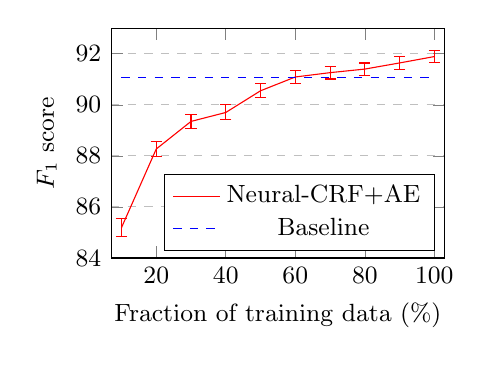
\begin{tikzpicture}
    \tikzstyle{every node}=[font=\small]

  \begin{axis}[
  	xlabel={Fraction of training data (\%)},
  	ylabel={$F_1$ score},
    xmin=7, xmax=103,
    ymin=84, ymax=93,
    height=4.5cm,
    ymajorgrids=true,
    grid style=dashed,
    width=0.48\textwidth,
    legend pos=south east
  ]

  \addplot[color=red, error bars/.cd, y dir=both, y explicit] coordinates {
  (10, 85.19)+=(10, 0.34)-=(10, 0.34)
  (20, 88.27)+=(20, 0.29)-=(20, 0.29)
  (30, 89.35)+=(30, 0.28)-=(30, 0.28)
  (40, 89.70)+=(40, 0.30)-=(40, 0.29)
  (50, 90.55)+=(50, 0.27)-=(50, 0.27)
  (60, 91.09)+=(60, 0.26)-=(60, 0.26)
  (70, 91.26)+=(70, 0.25)-=(70, 0.25)
  (80, 91.40)+=(80, 0.24)-=(80, 0.24)
  (90, 91.64)+=(90, 0.25)-=(90, 0.25)
  (100, 91.89)+=(100, 0.23)-=(100, 0.23)
  };
  \addlegendentry{Neural-CRF+AE}
  \addplot[blue, dashed] coordinates{(10,91.06)(100, 91.06)};
  \addlegendentry{Baseline}
  \end{axis}
\end{tikzpicture}

\vspace{-2ex}
\caption{Comparing the Neural-CRF+AE (red solid line) trained with varying amounts of data vs.\@ a Neural-CRF baseline (blue dashed line), trained on the full training set. Performance averaged over 5 runs, and error bars show $\pm$ 1 std.\@dev.}
\label{figure2}
\end{figure}

Neural systems typically require a large amount of annotated data.
Here we measure the impact of training with varying amount of annotated data,  as shown in  \figref{figure2}.
Wtih the proposed model architecture, the amount of labelled training data can be drastically reduced:
our model, achieves comparable performance against the baseline Neural-CRF, with as little as 60\% of the training data. 
Moreover, as we increase the amount of training text, the performance of Neural-CRF+AE continues to improve.
